\documentclass[12pt,english]{scrartcl}

\usepackage{amsmath,amssymb}
%\usepackage[amssymb]{SIunits}
\usepackage{babel}
\usepackage[latin1]{inputenc}
\usepackage{graphicx}
\usepackage{color}
\usepackage{url}


\begin{document}

\begin{center}
\textbf{\begin{LARGE}KOGW-PM-KNP:\\ \vspace{3mm} Tutorial 9 - Grasping
\end{LARGE}}
\end{center}

This tutorial deals with object manipulation performance. The paper by Wunsch et al., (2014) studies second-order motion planning in children of different age groups and compares it to performance in human adults and in cotton-top tamarin monkeys (see Fig. \ref{fig:tamarin}). Please read the paper carefully. Answer the following questions which should help you to evaluate the findings. Please work in pairs. 
 
\begin{figure}[htbp]
\begin{center}
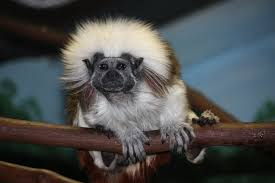
\includegraphics[width = 0.5\textwidth]{../../Slides/figs/l9/cotton_top_tamarin.jpg}
\end{center}
\caption{Cotton-top tamarin monkey
\label{fig:tamarin}}
\end{figure}

\begin{enumerate}
 \item What is involved in motor planning? What is meant by second-order motor planning? What is the end-state comfort (ESC) effect?

  \item How is ESC studied experimentally? What is the evidence as to when ESC effects emerge during development?

 \item How do monkeys (cotton-top tamarins and lemurs) perform on these tasks? Why is their performance surprising?

\item What factor do the authors suggest to be potentially responsible for the putative discrepancy?

\item What hypothesis did the authors test in the present experiment? What is the alternative hypothesis?

\item Describe the present experiment, design, independent, dependent, control variables

\item What is the main result of this study?

\item What do the authors conclude from their results? What kind of explanations do they offer? What do you find plausible?

\end{enumerate}

\end{document}
